\chapter{Analisa Sistem Tak Ubah Waktu}

\section*{Pengantar}
Pada bab-bab sebelumnya telah dibahas berbagai konsep matematika dasar: fungsi (Bab~2), interpolasi (Bab~4), kalkulus (Bab~5), dan Deret Fourier (Bab~6). Pada bab ini, semua konsep tersebut dipadukan dalam kerangka \textbf{Analisa Sistem Linier Tak Ubah Waktu} (LTW). Sinyal masukan dan keluaran merupakan \textit{fungsi} waktu, respon sistem dihitung melalui \textit{integral} konvolusi, dan Deret Fourier menyediakan representasi frekuensi dari sinyal periodik. Pemahaman tentang sifat fungsi (genap-ganjil, periodik, eksponensial) yang telah dipelajari pada Bab~2 akan sangat membantu dalam mengklasifikasikan dan menganalisis sinyal.

Sinyal dan sistem merupakan sebuah kesatuan yang saling berhubungan satu sama lain. Sinyal merupakan pola-pola bervariasi yang berubah terhadap satu atau lebih variabel bebas, yang berisi informasi tentang perilaku atau sifat dari suatu fenomena tertentu. Sistem akan menerima sinyal untuk kemudian mengelola, mengolahnya sehingga menghasilkan keluaran atau tanggapan berupa sinyal lain ataupun perilaku atau sifat tertentu sesuai keinginan. Penerapan sinyal dan sistem ada dalam banyak bidang yang bervariasi mulai dari teknologi komunikasi, elektronika, komputer, pembangkit energi, pengolahan suara untuk musik, transportasi, sampai kendali otomatis pada proses-proses di industri. Masih banyak lagi penerapan sinyal dan sistem dalam kehidupan sehari-hari yang kita sadari atau tidak telah kita gunakan secara rutin dalam kehidupan kita. Penerapan-penerapan tersebut kesemuanya memiliki pola dan ciri mendasar seperti yang telah dijabarkan pada awal paragraf. Contoh sederhananya adalah mobil. Mobil bergerak dan melaju dengan kecepatan tertentu akibat adanya injakan dari pedal gas, dalam hal ini injakan pada pedal gas merupakan sinyal masukan bagi sistem mobil dan sistem mobil melalui proses mekanis dan termodinamik pada mesinnya akan menghasilkan tanggapan berupa laju mobil yang sesuai dengan seberapa dalam injakan pedal gas. Contoh lain terdapat pada rangkaian listrik, dimana sinyal masukan berupa arus dan tegangan listrik yang berubah terhadap waktu pada sistem rangkaian listrik yang dapat berupa komponen-komponen elektronik dan elektrik seperti resistor, kapasitor dan lain-lain akan menghasilkan tanggapan berupa arus dan tegangan yang berbeda sesuai dengan yang diinginkan. 

\begin{figure}[!h]
\centering
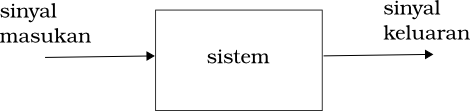
\includegraphics[scale=0.7]{pict/sinyalsistem}
\caption{Representasi konsep sinyal dan sistem dalam diagram blok}\label{sinyalsistem}
\end{figure}

Konsep sinyal dan sistem muncul dalam berbagai aplikasi yang berbeda bergantung pada bagaimana penggunaan konsep tersebut. Konsep sinyal dan sistem dapat digunakan untuk mengkarakterisasi sebuah sistem. Mengkarakterisasi berarti membaca karakter atau sifat dari sebuah sistem tertentu dengan cara memberikan sinyal masukan yang bervariasi dan membaca bagaimana sistem menanggapi masukan yang bervariasi tersebut. Hal ini seperti apabila kita mempunyai sebuah kotak hitam yang kita tidak tahu seperti apa sifat dan bagaimana kotak hitam tersebut bekerja. Dengan memberikan masukan bervariasi terhadap kotak hitam tersebut maka akan dapat diperoleh keluaran berupa tanggapan yang berbeda dengan masukan, sehingga dengan ini kita dapat mengetahui apa dan bagaimana kotak hitam misterius ini berperilaku atau bekerja. Konsep sinyal dan sistem juga dapat digunakan untuk melakukan pemrosesan terhadap sinyal tertentu agar diperoleh keluaran sinyal sesuai yang diharapkan atau untuk menghilangkan sinyal yang tidak diinginkan. Contohnya adalah dalam sistem \textit{noise canceling} (NC) atau pembatal bising. Dalam sistem NC yang biasa digunakan pada speaker, bising atau suara mengganggu yang tidak diinginkan dapat diredam sedemikian rupa sehingga suara atau bunyi yang keluar dari \textit{speaker} hanya suara yang diharapkan. Sistem NC akan membangkitkan suara dengan frekuensi tertentu yang sama dengan suara bising tertentu tetapi dengan fase yang berbeda sehingga melalui proses interferensi suara bising dapat diredam.

Sebelum membahas sifat-sifat sistem secara lebih mendalam, pada bagian berikut terlebih dahulu ditinjau berbagai jenis sinyal dan operasi yang dapat dilakukan terhadap sinyal. Pemahaman yang baik tentang representasi sinyal merupakan landasan penting untuk analisis sistem LTW.

\section{Representasi Sinyal}

Sinyal dapat diklasifikasikan berdasarkan variabel bebasnya. Sinyal \textbf{waktu-kontinu} $x(t)$ terdefinisi untuk setiap nilai $t$ pada suatu interval kontinu, sedangkan sinyal \textbf{waktu-diskrit} $x[n]$ hanya terdefinisi pada nilai-nilai bilangan bulat $n$ (sampel diskrit).

\begin{figure}[!h]
\centering
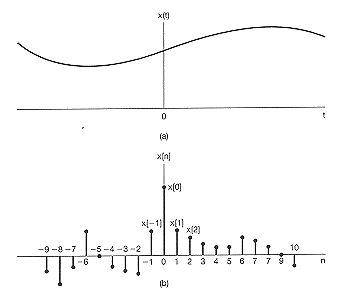
\includegraphics[scale=0.9]{pict/kontinudiskrit}
\caption{(a) Sinyal waktu-kontinu $x(t)$ dan (b) sinyal waktu-diskrit $x[n]$}\label{kontinudiskrit}
\end{figure}

\section{Transformasi Sinyal}
Konsep utama dalam analisa sinyal dan sistem adalah transformasi sinyal. Transformasi sinyal juga merupakan hal yang mendasar dan penting dalam pemrosesan sinyal terutama untuk melakukan manipulasi terhadap sinyal untuk menghilangkan sinyal yang tidak diinginkan ataupun menambahkan sesuatu pada sinyal sehingga menghasilkan sinyal yang sesuai dengan yang diinginkan. 
\subsection{Contoh-contoh transformasi variabel bebas}
Ada dua macam transformasi variabel bebas yang mendasar dan penting yaitu: pergeseran waktu (\textit{time shifting}) dan penskalaan waktu (\textit{time scaling}).
\begin{enumerate}
\item \textbf{pergeseran waktu}:\\
ambil sinyal waktu-kontinu $x(t)$, sinyal ini dapat digeser dengan pengurangan oleh faktor $t_0$
\[
x'(t)=x(t-t_0).
\] 
Jika $t_0>0$, sinyal $x(t)$ akan digeser ke kanan, atau terlambat (terjadi penundaan waktu/\textit{time delay}). Sedangkan jika $t_0<0$, maka $x(t)$ akan digeser ke kiri, atau mendahului. 

\begin{figure}[!h]
\centering
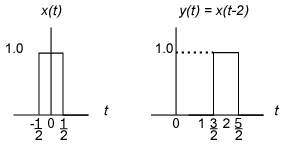
\includegraphics[scale=0.9]{pict/timeshift}
\caption{Gambaran operasi pergeseran waktu [2]}\label{timeshift}
\end{figure}

Untuk kasus sinyal diskrit $x[n]$, pergeseran waktu didefinisikan sebagai
\[
x'[n]=x[n-n_0],
\]
dengan $n_0$ yang juga harus merupakan bilangan bulat. Sama halnya dengan sinyal waktu-kontinu, jika $n_0$ positif maka sinyal tergeser ke kanan dan sebaliknya jika $n_0$ negatif maka sinyal tergeser ke kiri.

\item \textbf{penskalaan waktu}:\\
Sinyal yang didapatkan dengan menskalakan variabel bebas $t$ pada sinyal kontinu didefinisikan sebagai
\begin{equation}
x'(t)=x(at).
\end{equation} 
Untuk penskalaan waktu, jika $a>1$, maka sinyal akan terkompresi atau menyusut dari sinyal $x(t)$. Jika $0<a<1$, maka sinyal akan mengembang dari sinyal $x(t)$.

\begin{figure}[!h]
\centering
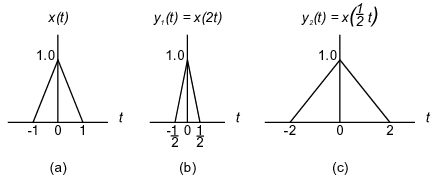
\includegraphics[scale=0.7]{pict/timescaling}
\caption{Operasi penskalaan waktu pada sinyal kontinu $x(t)$ [2]}
\end{figure}

\begin{figure}[!h]
\centering
\begin{subfigure}[b]{0.4\textwidth}
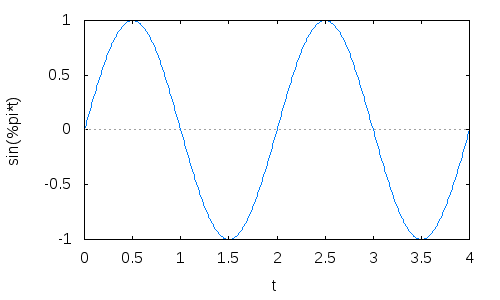
\includegraphics[width=\textwidth]{pict/timescaling1}
\caption{$x(t)=\sin \pi t$}
\end{subfigure}%
        ~ %add desired spacing between images, e. g. ~, \quad, \qquad etc.
          %(or a blank line to force the subfigure onto a new line)
\begin{subfigure}[b]{0.4\textwidth}
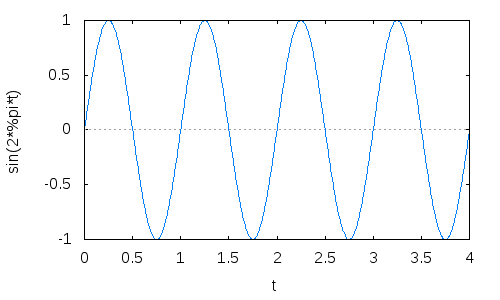
\includegraphics[width=\textwidth]{pict/timescaling2}
\caption{$x'_1(t)=\sin \pi 2t$}
\end{subfigure}
        ~ %add desired spacing between images, e. g. ~, \quad, \qquad etc.
          %(or a blank line to force the subfigure onto a new line)
\begin{subfigure}[b]{0.4\textwidth}
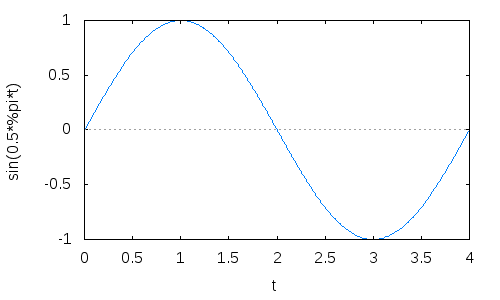
\includegraphics[width=\textwidth]{pict/timescaling3}
\caption{$x'_2(t)=\sin \pi \frac{t}{2}$}
\end{subfigure}
\caption{Efek penskalaan waktu pada sinyal sinusoidal}
\end{figure}

Untuk sinyal diskrit, penskalaan waktu didefinisikan sebagai
\begin{equation}
x'[n]=x[an]
\end{equation} 
\end{enumerate}
\subsection{Sinyal periodik}
Kelas sinyal penting yang akan sering kita jumpai dalam pemrosesan sinyal adalah sinyal periodik. Sinyal waktu-kontinu periodik $x(t)$ mempunyai sifat bahwa harga $T$-nya positif bagi
\begin{equation}
x(t) = x(t+T)
\end{equation}
untuk semua harga $t$. Sinyal periodik mempunyai sifat penting yaitu tidak berubah dengan pergeseran waktu $T$. Dalam persamaan (2.3) dikatakan bahwa $x(t)$ periodik dengan periode $T$. Jika $x(t)$ periodik dengan periode $T$, maka juga bisa dikatakan bahwa $x(t)=x(t+mT)$ untuk semua $t$ dan setiap bilangan bulat $m$. Dengan kata lain, $x(t)$ juga periodik dengan periode $2T, 3T, 4T, ...$ Periode dasar $T_0$ pada $x(t)$ merupakan harga positif terkecil $T$.

\begin{figure}[!h]
\centering
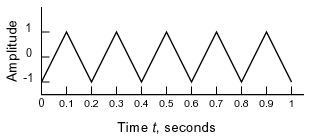
\includegraphics[scale=0.9]{pict/periodik}
\caption{Contoh sinyal periodik waktu-kontinu}
\end{figure}

Sinyal periodik pada waktu-diskrit didefinisikan sebagai
\begin{equation}
x[n]=x[n+N].
\end{equation}
Sinyal waktu diskrit $x[n]$ adalah periodik dengan periode $N$, dengan $N$ adalah bilangan bulat positif. 

\subsection{Sinyal genap dan sinyal ganjil}
Sinyal $x(n)$ atau $x[n]$ dikatakan sebagai sinyal genap jika identik terhadap waktu balikannya identik. Seperti bayangan pada cermin. Untuk sinyal waktu-kontinu didefinisikan sebagai
\begin{equation}
x(-t) = x(t),
\end{equation}
sedangkan untuk waktu-diskrit didefinisikan sebagai
\begin{equation}
x[-n]=x[n].
\end{equation}
Sinyal dikatakan sebagai sinyal ganjil jika
\begin{align}
x(-t) &= -x(t)\\
x[-n] &= -x[n].
\end{align}  
Sinyal ganjil harus 0 jika $x=0$ atau $n=0$.
\begin{figure}
\centering
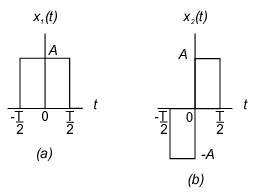
\includegraphics[scale=0.9]{pict/genapganjil}
\caption{Contoh sinyal genap (a) dan ganjil (b).}
\end{figure} 

\section{Sinyal Eksponensial dan Sinyal Sinusoidal Waktu-kontinu}
Sinyal eksponensial waktu-kontinu didefinisikan dalam bentuk umum
\begin{equation}
x(t)=Ce^{at}.
\end{equation}
Ada beberapa karakteristik berbeda yang dapat ditampilkan oleh sinyal eksponensial bergantung pada parameter $C$ dan $a$ yang dimilikinya, Karakteristik-karakteristik ini ditampilkan pada tabel 2.1 berikut

\begin{table}
\centering
\caption{Beberapa karakteristik sinyal eksponensial kompleks}
\begin{tabular}{|c|c|c|}
\hline
\textbf{Karakteristik} & $C$ & $a$\\
\hline
\hline
Sinyal eksponensial real & real & real\\
\hline
Sinyal eksponensial kompleks periodik & real & imajiner\\
\hline
Sinyal eksponensial kompleks umum & kompleks & kompleks\\
\hline
\end{tabular}
\end{table}
\subsection{Sinyal eksponensial real}
Sinyal eksponensial real mempunyai komponen $C$ dan $a$ berupa bilangan real. Bergantung pada apakah nilai $a$ positif atau negatif, sinyal eksponensial real terbagi menjadi sinyal eksponensial meningkat dan sinyal eksponensial meluruh.
\[
a>0\;\;\rightarrow \text{sinyal eksponensial meningkat}
\]
\[
a<0\;\;\rightarrow \text{sinyal eksponensial meluruh}
\]
\begin{figure}[!h]
\centering
\begin{subfigure}[b]{0.4\textwidth}
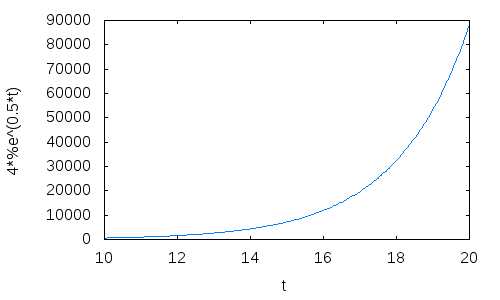
\includegraphics[width=\textwidth]{pict/exponensial1}
\caption{$x_1(t)=4e^{0.5t}$}
\end{subfigure}%
\begin{subfigure}[b]{0.4\textwidth}
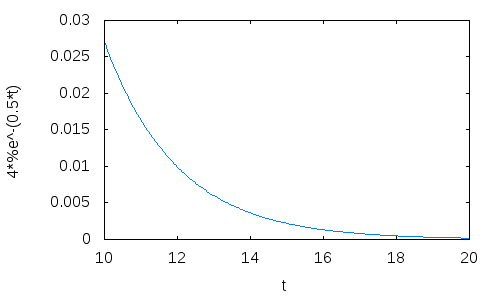
\includegraphics[width=\textwidth]{pict/exponensial2}
\caption{$x_2(t)=4e^{-0.5t}$}
\end{subfigure}
\caption{Sinyal eksponensial meningkat (a) dan sinyal eksponensial meluruh (b)}
\end{figure}

\subsection{Sinyal eksponensial kompleks periodik}
Sinyal eksponensial kompleks periodik memiliki komponen $a$ yang imajiner. 
\begin{equation}
x(t)=e^{j\omega_0 t}
\end{equation}
Sinyal jenis ini bersifat periodik, jika kita tengok kembali persamaan (2.3) maka didapat bahwa
\[
e^{j\omega_0 t}=e^{j\omega_0 (t+T)}
\]
atau
\[
e^{j\omega_0(t+T)}=e^{j\omega_0 t} e^{j\omega_0 T}.
\]
Dari sini kita lihat bahwa suatu sinyal periodik jika 
\[
e^{j\omega_0 T} = 1.
\]
Sinyal eksponensial periodik memiliki periode dasar $T_0$,
\begin{equation}
T_0=\frac{2\pi}{|\omega_0|}.
\end{equation}
Sinyal $e^{j\omega_0 t}$ dan $e^{-j\omega_0 t}$ mempunyai periode dasar yang sama.

\subsection{Sinyal sinusoidal}
Secara umum sinyal sinusoidal didefinisikan sebagai
\begin{equation}
x(t) = A \cos (\omega_0 t + \phi),
\end{equation}
dengan $A$ adalah amplituda sinyal, $\omega_0$ adalah frekuensi sudut dengan satuan radian per sekon, dan $\phi$ adalah fase dengan satuan radian. $\omega_0$ dapat ditulis sebagai
\[
\omega_0=2 \pi f_0,
\]
dengan $f_0$ adalah frekuensi dasar yang memiliki satuan putaran per sekon. Sinyal sinusoidal adalah sinyal periodik dengan periode dasar $T_0$. Sinyal sinusoidal memiliki hubungan dengan sinyal eksponensial periodik melalui hubungan Euler
\begin{equation}
e^{j\omega_0 t}=\cos \omega_0 t + j \sin \omega_0 t.
\end{equation}
Kita bisa mengekspresikan sinyal sinusoidal ke dalam komponen real dan imajiner eksponensial kompleksnya.
\begin{align}
A\cos (\omega_0 t+\phi)&=A \Re\lbrace e^{(j\omega_0t+\phi)}\rbrace\\
A\sin (\omega_0 t +\phi)&= A\Im\lbrace e^{(j\omega_0 t+\phi)}\rbrace. 
\end{align}
Selain itu, sinyal sinusoidal juga dapat dituliskan ke dalam sinyal eksponensial periodik melalui
\begin{equation}
A\cos (\omega_0 t+\phi)=\frac{A}{2}e^{j\phi}e^{j\omega_0 t} + \frac{A}{2} e^{-j \phi} e^{-j\omega_0 t}. 
\end{equation} 

\begin{figure}
\centering
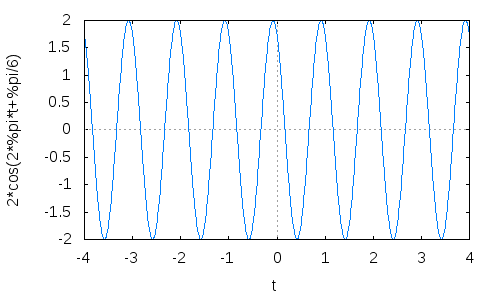
\includegraphics[scale=0.4]{pict/sinusoidal}
\caption{Contoh sinyal sinusoidal $x(t)=2\cos (2\pi t+\frac{\pi}{6})$}
\end{figure}

\subsection{Sinyal eksponensial kompleks umum}
Sinyal eksponensial kompleks umum memilik komponen $C$ dan $a$ berupa bilangan kompleks. Dalam hal ini $C$ diekspresikan ke dalam bentuk polar ($re^{j \phi}$), sedangkan $a$ ke dalam bentuk rektangular ($x+jy$). 
\begin{align*}
C&=|C|e^{j\phi}\\
a&=r+j\omega_0.
\end{align*}
Maka sinyal eksponensial kompleks umum dituliskan sebagai
\begin{equation}
Ce^{at}=|C|e^{j\phi}e^{(r+j\omega_0)}=|C|e^{rt}e^{j(\omega_0 t+\phi)}.
\end{equation}
Dengan menggunakan hubungan Euler, kita dapat memperluasnya menjadi
\begin{equation}
Ce^{at}=|C|e^{rt} \cos(\omega_0 t+\phi)+j|C|e^{rt}\sin(\omega_0 t+\phi).
\end{equation}
Untuk nilai $r$, jika
\begin{align*}
r=0\;\;&\rightarrow \text{bagian real dan imajiner eksponensial kompleks adalah sinusoidal}\\
r>0\;\;&\rightarrow \text{sinyal sinusoidal meningkat}\\
r<0\;\;&\rightarrow \text{sinyal sinusoidal meluruh atau teredam}
\end{align*}

\section{Sinyal Eksponensial Kompleks dan Sinyal Sinusoidal Kompleks Waktu-Diskrit}

Analog dengan kasus waktu-kontinu, sinyal eksponensial kompleks waktu-diskrit didefinisikan sebagai
\begin{equation}
x[n] = C\alpha^n,
\end{equation}
dengan $C$ dan $\alpha$ pada umumnya berupa bilangan kompleks. Bentuk ini ekivalen dengan $x[n] = Ce^{\beta n}$ jika $\alpha = e^\beta$.

\subsection{Sinyal eksponensial real waktu-diskrit}

Jika $C$ dan $\alpha$ berupa bilangan real, maka $x[n] = C\alpha^n$ adalah sinyal eksponensial real. Perilaku sinyal bergantung pada nilai $\alpha$:
\begin{align*}
|\alpha| > 1 \;\;&\rightarrow \text{sinyal eksponensial meningkat}\\
|\alpha| < 1 \;\;&\rightarrow \text{sinyal eksponensial meluruh}\\
\alpha > 0    \;\;&\rightarrow \text{semua sampel bertanda sama (tidak berganti tanda)}\\
\alpha < 0    \;\;&\rightarrow \text{tanda sampel berganti-ganti (osilasi bolak-balik)}
\end{align*}

\begin{exmp}
Tentukan sifat sinyal $x[n] = (0{,}5)^n$ dan $x[n] = (-0{,}5)^n$!

\textbf{Penyelesaian:}\\
Untuk $\alpha = 0{,}5$: karena $|\alpha| < 1$ dan $\alpha > 0$, sinyal meluruh dengan semua sampel positif.\\
Untuk $\alpha = -0{,}5$: karena $|\alpha| < 1$ dan $\alpha < 0$, sinyal meluruh namun tanda sampel berganti-ganti: $1,\,-0{,}5,\,0{,}25,\,-0{,}125,\,\ldots$
\end{exmp}

\subsection{Sinyal eksponensial kompleks periodik waktu-diskrit}

Sinyal eksponensial kompleks waktu-diskrit dengan parameter $\alpha$ pada lingkaran satuan ($|\alpha|=1$) didefinisikan sebagai
\begin{equation}
x[n] = e^{j\omega_0 n},
\end{equation}
dengan $\omega_0$ adalah frekuensi sudut diskrit dalam satuan radian per sampel.

\textbf{Perbedaan penting dengan waktu-kontinu:} Pada kasus waktu-kontinu, $e^{j\omega_0 t}$ selalu periodik untuk sebarang $\omega_0 \ne 0$. Namun pada kasus waktu-diskrit, $e^{j\omega_0 n}$ \textit{periodik dengan periode bulat $N$} jika dan hanya jika terdapat bilangan bulat positif $N$ sedemikian sehingga
\begin{equation}
e^{j\omega_0(n+N)} = e^{j\omega_0 n},
\end{equation}
yang berarti $e^{j\omega_0 N} = 1$, sehingga $\omega_0 N = 2\pi m$ untuk suatu bilangan bulat $m$. Dengan demikian,
\begin{equation}
\frac{\omega_0}{2\pi} = \frac{m}{N}.
\end{equation}
Syarat keperiodikan: $e^{j\omega_0 n}$ periodik jika dan hanya jika $\omega_0 / (2\pi)$ merupakan bilangan rasional. Periode dasar $N_0$ adalah nilai terkecil $N$ yang memenuhi syarat tersebut.

\textbf{Perbedaan penting lainnya:} Sinyal waktu-diskrit $e^{j\omega_0 n}$ dan $e^{j(\omega_0 + 2\pi k)n}$ untuk sebarang bilangan bulat $k$ adalah identik, karena
\[
e^{j(\omega_0+2\pi k)n} = e^{j\omega_0 n}\cdot e^{j2\pi kn} = e^{j\omega_0 n}.
\]
Oleh karena itu, sinyal eksponensial kompleks waktu-diskrit dengan frekuensi berbeda yang terpisah sebesar kelipatan $2\pi$ adalah sinyal yang \textbf{sama}. Rentang frekuensi yang unik cukup diambil pada interval $0 \le \omega_0 < 2\pi$ atau $-\pi < \omega_0 \le \pi$.

\begin{exmp}
Tentukan apakah sinyal $x[n] = e^{j(3\pi/4)n}$ periodik, dan jika ya, tentukan periode dasarnya!

\textbf{Penyelesaian:}\\
Dengan $\omega_0 = 3\pi/4$, maka $\omega_0/(2\pi) = 3/8$, yang merupakan bilangan rasional ($m=3$, $N=8$). Jadi sinyal ini periodik dengan periode dasar $N_0 = 8$.
\end{exmp}

\begin{exmp}
Tentukan apakah sinyal $x[n] = e^{j\sqrt{2}\,n}$ periodik!

\textbf{Penyelesaian:}\\
Dengan $\omega_0 = \sqrt{2}$, maka $\omega_0/(2\pi) = \sqrt{2}/(2\pi)$, yang merupakan bilangan irasional. Jadi sinyal ini \textbf{tidak periodik}.
\end{exmp}

\subsection{Sinyal sinusoidal waktu-diskrit}

Sinyal sinusoidal waktu-diskrit didefinisikan sebagai
\begin{equation}
x[n] = A\cos(\omega_0 n + \phi),
\end{equation}
dengan $A$ adalah amplituda, $\omega_0$ adalah frekuensi sudut diskrit (radian per sampel), dan $\phi$ adalah fasa (radian). Melalui hubungan Euler, sinyal sinusoidal dapat dinyatakan dalam bentuk eksponensial kompleks:
\begin{equation}
A\cos(\omega_0 n + \phi) = \frac{A}{2}e^{j\phi}\,e^{j\omega_0 n} + \frac{A}{2}e^{-j\phi}\,e^{-j\omega_0 n}.
\end{equation}

Sebagaimana sinyal eksponensial kompleks, sinyal sinusoidal $A\cos(\omega_0 n + \phi)$ adalah periodik jika dan hanya jika $\omega_0/(2\pi)$ adalah bilangan rasional, dan frekuensi-frekuensi yang berbeda kelipatan $2\pi$ menghasilkan sinyal yang identik.

\subsection{Sinyal eksponensial kompleks umum waktu-diskrit}

Untuk kasus umum dengan $C = |C|e^{j\phi}$ dan $\alpha = |\alpha|e^{j\omega_0}$, sinyal eksponensial kompleks waktu-diskrit adalah
\begin{equation}
x[n] = C\alpha^n = |C|e^{j\phi}\,|\alpha|^n\,e^{j\omega_0 n} = |C|\,|\alpha|^n\,e^{j({\omega_0 n+\phi})}.
\end{equation}
Dengan menggunakan hubungan Euler, bagian real dan imajinernya adalah
\begin{align}
\Re\{x[n]\} &= |C|\,|\alpha|^n\cos(\omega_0 n + \phi),\\
\Im\{x[n]\} &= |C|\,|\alpha|^n\sin(\omega_0 n + \phi).
\end{align}
Perilaku amplitudo sinyal ditentukan oleh $|\alpha|$:
\begin{align*}
|\alpha| = 1 \;\;&\rightarrow \text{sinyal sinusoidal dengan amplituda tetap}\\
|\alpha| > 1 \;\;&\rightarrow \text{sinyal sinusoidal dengan amplituda meningkat}\\
|\alpha| < 1 \;\;&\rightarrow \text{sinyal sinusoidal dengan amplituda meluruh (teredam)}
\end{align*}


\section{Sistem Linear}

Sistem dikatakan \textbf{linear} jika memenuhi dua sifat dasar yaitu \textit{homogenitas} (penskalaan) dan \textit{aditivitas} (superposisi). Misalkan $y_1(t)$ adalah keluaran sistem untuk masukan $x_1(t)$, dan $y_2(t)$ adalah keluaran untuk masukan $x_2(t)$.

\begin{enumerate}
\item \textbf{Homogenitas (Penskalaan)}: Jika masukan dikalikan dengan sebuah konstanta $a$, maka keluaran juga akan dikalikan dengan konstanta yang sama, yaitu
\[
a\,x_1(t) \longrightarrow a\,y_1(t).
\]

\item \textbf{Aditivitas (Superposisi)}: Keluaran dari penjumlahan dua masukan sama dengan penjumlahan keluaran masing-masing masukan, yaitu
\[
x_1(t) + x_2(t) \longrightarrow y_1(t) + y_2(t).
\]
\end{enumerate}

Kedua sifat tersebut dapat digabungkan menjadi satu \textit{prinsip superposisi}: untuk sebarang konstanta $a$ dan $b$,
\begin{equation}
a\,x_1(t) + b\,x_2(t) \longrightarrow a\,y_1(t) + b\,y_2(t).
\label{eq:superposisi}
\end{equation}

Jika persamaan~\ref{eq:superposisi} berlaku untuk semua pilihan $a$, $b$, $x_1(t)$, dan $x_2(t)$, maka sistem tersebut adalah sistem linear. Jika tidak memenuhi salah satu sifat tersebut, sistem dikatakan \textit{nonlinear}.

\begin{exmp}
Tentukan apakah sistem dengan persamaan $y(t) = 2x(t) + 3$ linear atau tidak!

\textbf{Penyelesaian:}\\
Untuk masukan $x_1(t)$, keluarannya adalah $y_1(t) = 2x_1(t) + 3$.\\
Untuk masukan $x_2(t)$, keluarannya adalah $y_2(t) = 2x_2(t) + 3$.\\
Untuk masukan $a\,x_1(t) + b\,x_2(t)$, keluarannya adalah
\[
y(t) = 2\bigl(a\,x_1(t) + b\,x_2(t)\bigr) + 3 = a\,y_1(t) + b\,y_2(t) - 3(a+b-1).
\]
Karena $y(t) \ne a\,y_1(t) + b\,y_2(t)$ (kecuali $a+b=1$), sistem ini \textbf{tidak linear} (nonlinear) karena adanya konstanta aditif $3$ yang melanggar prinsip superposisi.
\end{exmp}

\begin{exmp}
Tentukan apakah sistem $y(t) = t\,x(t)$ linear atau tidak!

\textbf{Penyelesaian:}\\
Untuk masukan $a\,x_1(t) + b\,x_2(t)$, keluarannya adalah
\[
y(t) = t\bigl(a\,x_1(t)+b\,x_2(t)\bigr) = a\,t\,x_1(t) + b\,t\,x_2(t) = a\,y_1(t)+b\,y_2(t).
\]
Sistem ini memenuhi prinsip superposisi, sehingga sistem ini \textbf{linear}.
\end{exmp}

\section{Sistem Tak Ubah Waktu}

Sistem dikatakan \textbf{tak ubah waktu} (\textit{time-invariant}) jika karakteristik dan perilaku sistem tidak berubah terhadap waktu. Secara formal, jika $y(t)$ adalah keluaran sistem untuk masukan $x(t)$, maka untuk sebarang penundaan waktu $t_0$, berlaku
\begin{equation}
x(t - t_0) \longrightarrow y(t - t_0).
\label{eq:tak-ubah-waktu}
\end{equation}
Dengan kata lain, penundaan pada masukan menghasilkan penundaan yang sama pada keluaran. Jika sifat ini tidak terpenuhi, sistem dikatakan \textit{ubah waktu} (\textit{time-varying}).

Sistem yang bersifat linear \textit{dan} tak ubah waktu secara bersama-sama disebut sistem \textbf{Linear Tak Ubah Waktu} (LTW), atau dalam bahasa Inggris \textit{Linear Time-Invariant} (LTI). Sistem LTW memiliki sifat yang sangat berguna karena dapat dianalisis sepenuhnya melalui respon impulsnya.

\begin{exmp}
Tentukan apakah sistem $y(t) = x(t)\cos(\omega_0 t)$ merupakan sistem tak ubah waktu!

\textbf{Penyelesaian:}\\
Jika masukan digeser menjadi $x(t-t_0)$, keluaran sistem adalah
\[
y_1(t) = x(t-t_0)\cos(\omega_0 t).
\]
Sedangkan keluaran yang digeser adalah
\[
y(t-t_0) = x(t-t_0)\cos\bigl(\omega_0(t-t_0)\bigr).
\]
Karena $y_1(t) \ne y(t-t_0)$ (faktor kosinus berbeda), maka sistem ini \textbf{ubah waktu} (time-varying).
\end{exmp}

\section{Respon Impuls dan Konvolusi}

\subsection{Fungsi Impuls (Delta Dirac)}

Fungsi impuls satuan, atau \textit{fungsi delta Dirac} $\delta(t)$, merupakan sinyal yang sangat penting dalam analisis sistem. Fungsi ini didefinisikan melalui sifat-sifatnya:
\begin{equation}
\delta(t) = 0, \quad t \ne 0,
\end{equation}
\begin{equation}
\int_{-\infty}^{\infty} \delta(t)\,dt = 1.
\end{equation}

Sifat yang paling berguna dari fungsi delta Dirac adalah \textit{sifat pengambilan sampel} (\textit{sifting property}):
\begin{equation}
\int_{-\infty}^{\infty} x(t)\,\delta(t - t_0)\,dt = x(t_0).
\label{eq:sifting}
\end{equation}
Persamaan~\ref{eq:sifting} menyatakan bahwa pengintegralan suatu fungsi $x(t)$ dikalikan $\delta(t-t_0)$ menghasilkan nilai fungsi tersebut di titik $t=t_0$.

Untuk sinyal diskrit, padanan fungsi impuls adalah \textit{impuls satuan} $\delta[n]$, yang didefinisikan sebagai
\begin{equation}
\delta[n] = \begin{cases} 1, & n = 0 \\ 0, & n \ne 0. \end{cases}
\end{equation}

\subsection{Respon Impuls}

\textbf{Respon impuls} $h(t)$ dari suatu sistem LTW adalah keluaran sistem ketika masukannya adalah impuls satuan $\delta(t)$, dengan asumsi kondisi awal nol:
\begin{equation}
\delta(t) \longrightarrow h(t).
\end{equation}
Respon impuls sepenuhnya mendeskripsikan perilaku sistem LTW. Artinya, jika kita mengetahui $h(t)$, kita dapat menghitung keluaran sistem untuk masukan \textit{apapun}.

\subsection{Konvolusi}

Sembarang sinyal masukan kontinu $x(t)$ dapat dinyatakan sebagai superposisi impuls yang bergeser:
\begin{equation}
x(t) = \int_{-\infty}^{\infty} x(\tau)\,\delta(t-\tau)\,d\tau.
\end{equation}
Dengan menggunakan linieritas dan sifat tak ubah waktu, keluaran sistem LTW untuk masukan $x(t)$ adalah
\begin{equation}
y(t) = \int_{-\infty}^{\infty} x(\tau)\,h(t-\tau)\,d\tau.
\label{eq:konvolusi}
\end{equation}
Operasi pada persamaan~\ref{eq:konvolusi} disebut \textbf{konvolusi} (atau lebih lengkap, konvolusi linier) dan dinyatakan dengan tanda bintang:
\begin{equation}
y(t) = x(t) * h(t).
\end{equation}

Untuk sistem LTW waktu-diskrit, konvolusi didefinisikan sebagai
\begin{equation}
y[n] = \sum_{k=-\infty}^{\infty} x[k]\,h[n-k] = x[n] * h[n].
\end{equation}

\subsection{Sifat-sifat Konvolusi}

Konvolusi memiliki beberapa sifat penting:
\begin{enumerate}
\item \textbf{Komutatif}: $x(t)*h(t) = h(t)*x(t)$
\item \textbf{Asosiatif}: $\bigl(x(t)*h_1(t)\bigr)*h_2(t) = x(t)*\bigl(h_1(t)*h_2(t)\bigr)$
\item \textbf{Distributif terhadap penjumlahan}: $x(t)*\bigl(h_1(t)+h_2(t)\bigr) = x(t)*h_1(t) + x(t)*h_2(t)$
\end{enumerate}

\begin{exmp}
Hitunglah konvolusi $y[n] = x[n] * h[n]$ jika
\[
x[n] = \{1,\, 2,\, 1\}, \quad h[n] = \{1,\, 1,\, 1\},
\]
dengan indeks dimulai dari $n = 0$.

\textbf{Penyelesaian:}\\
Menggunakan definisi konvolusi:
\begin{align*}
y[0] &= x[0]h[0] = 1 \cdot 1 = 1\\
y[1] &= x[0]h[1] + x[1]h[0] = 1\cdot 1 + 2\cdot 1 = 3\\
y[2] &= x[0]h[2] + x[1]h[1] + x[2]h[0] = 1 + 2 + 1 = 4\\
y[3] &= x[1]h[2] + x[2]h[1] = 2\cdot 1 + 1\cdot 1 = 3\\
y[4] &= x[2]h[2] = 1\cdot 1 = 1
\end{align*}
Sehingga $y[n] = \{1,\, 3,\, 4,\, 3,\, 1\}$.
\end{exmp}

\section{Kausalitas}

Sistem dikatakan \textbf{kausal} (\textit{causal}) jika keluarannya pada setiap saat $t_0$ hanya bergantung pada nilai masukan pada saat $t \le t_0$. Dengan kata lain, keluaran sistem tidak bergantung pada nilai masukan di masa mendatang. Semua sistem fisis yang beroperasi secara \textit{real-time} adalah kausal, karena sistem tersebut tidak dapat "mengetahui" masukan yang belum terjadi.

Secara matematis, sistem LTW waktu-kontinu adalah kausal jika dan hanya jika respon impulsnya memenuhi
\begin{equation}
h(t) = 0, \quad t < 0.
\end{equation}
Jika kondisi ini terpenuhi, integral konvolusi menjadi
\begin{equation}
y(t) = \int_{0}^{\infty} h(\tau)\,x(t-\tau)\,d\tau = \int_{-\infty}^{t} x(\tau)\,h(t-\tau)\,d\tau.
\end{equation}

Untuk sistem LTW waktu-diskrit, kondisi kausalitas adalah $h[n] = 0$ untuk $n < 0$.

\begin{exmp}
Tentukan apakah sistem berikut kausal atau tidak:
\begin{enumerate}
\item[(a)] $y(t) = x(t-1)$ \quad (penundaan waktu)
\item[(b)] $y(t) = x(t+1)$ \quad (maju waktu)
\item[(c)] $y(t) = x(-t)$ \quad (pembalikan waktu)
\end{enumerate}

\textbf{Penyelesaian:}\\
(a) Keluaran $y(t)$ bergantung pada $x(t-1)$, yaitu nilai masukan satu satuan \textit{sebelumnya}. Sistem ini \textbf{kausal}.\\
(b) Keluaran $y(t)$ bergantung pada $x(t+1)$, yaitu nilai masukan satu satuan di masa \textit{mendatang}. Sistem ini \textbf{tidak kausal} (\textit{anti-causal}).\\
(c) Keluaran $y(0)$ bergantung pada $x(0)$, tetapi $y(-1)$ bergantung pada $x(1)$ yaitu nilai masukan di masa mendatang. Sistem ini \textbf{tidak kausal}.
\end{exmp}

\section{Kestabilan}

Sistem dikatakan \textbf{stabil} dalam pengertian \textit{Bounded-Input Bounded-Output} (BIBO) jika setiap masukan yang terbatas menghasilkan keluaran yang terbatas. Secara formal, sistem stabil BIBO jika untuk setiap $|x(t)| \le M_x < \infty$, terdapat $M_y < \infty$ sedemikian sehingga $|y(t)| \le M_y$ untuk semua $t$.

Untuk sistem LTW waktu-kontinu, syarat perlu dan cukup agar sistem stabil BIBO adalah
\begin{equation}
\int_{-\infty}^{\infty} |h(\tau)|\,d\tau < \infty,
\end{equation}
yaitu respon impuls harus \textit{mutlak dapat diintegralkan}. Untuk sistem LTW waktu-diskrit, syarat yang ekivalen adalah
\begin{equation}
\sum_{k=-\infty}^{\infty} |h[k]| < \infty.
\end{equation}



\section*{Rangkuman}

Pada bab ini telah dibahas konsep-konsep dasar analisis sinyal dan sistem Linier Tak Ubah Waktu (LTW). Sinyal dapat berupa waktu-kontinu atau waktu-diskrit, dan dapat diklasifikasikan berdasarkan sifat periodik, genap-ganjil, maupun jenis eksponensialnya. Operasi transformasi sinyal meliputi pergeseran waktu, penskalaan waktu, dan pembalikan waktu.

Sistem LTW didefinisikan oleh dua sifat utama: \textit{linieritas} (prinsip superposisi) dan \textit{ketakinvarianan waktu}. Setiap sistem LTW dapat dideskripsikan sepenuhnya oleh \textbf{respon impulsnya} $h(t)$, sehingga keluaran untuk sembarang masukan $x(t)$ diperoleh melalui operasi \textbf{konvolusi}:
\[
y(t) = x(t) * h(t) = \int_{-\infty}^{\infty} x(\tau)\,h(t-\tau)\,d\tau.
\]
Dua sifat penting yang menentukan kelayakan sistem untuk implementasi nyata adalah \textbf{kausalitas} (keluaran hanya bergantung pada nilai masukan masa kini dan lampau) dan \textbf{kestabilan BIBO} (masukan terbatas menghasilkan keluaran yang terbatas).

\section*{Latihan Soal}

\begin{enumerate}
  \item Tentukan apakah sistem-sistem berikut linear, tak ubah waktu, kausal, dan/atau stabil BIBO:
  \begin{enumerate}[(a)]
    \item $y(t) = x(t-2) + x(t+1)$
    \item $y(t) = x^2(t)$
    \item $y[n] = \displaystyle\sum_{k=0}^{n} x[k]$
  \end{enumerate}
  \item Hitunglah konvolusi $y[n] = x[n] * h[n]$ untuk $x[n] = \{3,\,1,\,2\}$ dan $h[n] = \{1,\,2,\,1\}$, dengan indeks dimulai dari $n=0$!
  \item Buktikan bahwa sistem dengan $h(t) = e^{-2t}u(t)$ (di mana $u(t)$ adalah fungsi tangga satuan) adalah sistem yang stabil BIBO dan kausal!
  \item Tentukan apakah sinyal-sinyal berikut periodik, dan jika periodik, tentukan periode dasarnya:
  \begin{enumerate}[(a)]
    \item $x(t) = \cos(3\pi t) + \sin(5\pi t)$
    \item $x[n] = e^{j(2\pi/5)n} + e^{j(7\pi/3)n}$
  \end{enumerate}
\end{enumerate}
